\chapter{Artificial intelligence \& Machine Learning}

Machine learning is a branch of \Gls{ai}. 
The field of \Gls{machinevision} is a branch of machine vision in which important steps forward has been made in the past decade, mainly thanks to the emergence of \Gls{deepl}.

The aim of this chapter is not to provide a complete overview of the machine learning field.
Rather, the objective is to highlight concepts that are important for interpretation of the specific analysis in this Master thesis.

\section{Birds-eye view on the field of Artificial Intelligence}

The field of \Gls{ai} (AI) is the engineering discipline of the automation of \textit{cognitive} tasks.
Tasks such as search, control and classification are generally considered to require a level of intelligence. 
Automation of this type of tasks to allow a machine to perform them is thus \Gls{ai}\footnote{To be precise, it is not the human intelligence that is replicated. It is the \textit{effect} of this intelligence.}.
A classic PID controller and even a bang-bang (thermostat) controller can be viewed as simple, but very effective, forms of AI.


In the past decades, this engineering discipline has incredible advance, driven both by leaps forward in the available hardware and the development of new algorithms and models. \\
First, the availability and reliability of hardware components such as sensors, cameras, digital storage and calculation power has increased exponentially 
\footnote{ \textit{Moore's law} states that the number of transistors on an integrated curcuit doubles every two years. This rate of progress has held more of less for a wide range of digital components in the past decades.}.
The size and price of these components has decreased equally dramatically. \\
Second, important progress has been made in the development of algorithms to make use of this available data and computation power to solve problems and perform tasks.
I do not want to provide a complete overview of all existing machine learning models. 
In this work, I make use of \Gls{deepl} models.
A \Gls{deepl} model is a type of \acrfull{ann} with multiple hidden layers. 
Deep learning models are behind almost all modern applications of \acrfull{nlp} and \Gls{machinevision}.

Deep learning models can be fitted through the \acrfull{bp} algorithm. 
\todo[inline]{Short and to-the point introduction of neural networks}

\section{Losses and metrics}

Constructing a network requires evaluating it. 
A network is fitted to the \textit{train set} by the optimization algorithm, based on the \textbf{loss}.
The \acrshort{ml} engineer wants to judge the performance of the model based on one or several \textbf{metrics}, calculated on the \textit{train set}, the \textit{cross-validation set} and eventually on the \textit{test set}.

\subsection{Loss functions}

To fit a model, the optimizer will minimize the loss function.
To use the gradient descent algorithm, this loss function needs to be a differentiable function.

The (binary) cross-entropy loss over $N$ datapoints with true value $t_i \in \left\{0;1\right\}$ and softmax probability $0 \leq p_i \leq 1$ ($i\in \{0;..;N-1\}$) is defined as 
\begin{equation}
    \mathcal{L} = -\frac{1}{N} \left(  
        \sum^{N-1}_{i=0} \left(
            t_i log(p_i) + (1 - t_i) log( 1 - p_i )
        \right)
     \right)
\end{equation}

\subsection{Metrics}

Metrics are used to evaluate and compare \acrlong{ml} models.
Numerous metrics are possible, I will focus on the important metrics used for multi-class classificiation problems.
\marginpar{
% Please add the following required packages to your document preamble:
% \usepackage{multirow}
%\begin{table}[]
    \begin{tabular}{cllll}
    \hline
    \multicolumn{1}{l}{}                &                        & \multicolumn{3}{l}{\textbf{Actual class}}           \\
    \multicolumn{1}{l}{}                &                        & $C_0$   & $C_1$   & $C_2$                        \\ \cline{3-5} 
    \multirow{3}{*}{\rotatebox[origin=c]{90}{\parbox[c]{1cm}{\centering \textbf{Predicted class}}}}   & \multicolumn{1}{l|}{$C_0$} & $a_{0,0}$ & $a_{0,1}$ & \multicolumn{1}{l|}{$a_{0,2}$} \\
                                        & \multicolumn{1}{l|}{$C_1$} & $a_{1,0}$ & $a_{1,1}$  & \multicolumn{1}{l|}{$a_{1,2}$ } \\
                                        & \multicolumn{1}{l|}{$C_2$} & $a_{2,0}$  & $a_{2,1}$  & \multicolumn{1}{l|}{$a_{2,2}$ } \\ \hline
    \end{tabular}
    %\end{table}

    \captionof{table}{Illustration of confusion matrix with 3 classes.}
    \label{tab:confusionMatrix}
    }

Table \ref{tab:confusionMatrix} illustrates a confusion matrix for a model for a problem with 3 classes ($C_j:j\in \{1;2;3\}$). 
A model predicts the class for all observations in the set.
The confusion matrix allows to compare these preditions against the true class\footnote{The true class is the label for this observation.}.

$a_{0,0}$, $a_{1,1}$, $a_{2,2}$ are the correctly labelled observations. 
The predicted class corresponds to the actual class.
This is not necessarily the case for all observations. For example, $a_{1,2}$ observations with true class $C_2$ the model predicted to belong to class $C_1$.
In general $a_{i,j}$ is the number of observations for which the model predicted $C_i$ and for which the label is $C_j$.
Based on the confusion matrix, 3 metrics can be calculated: the model \textit{precision}, the \textit{recall} and the \textit{F-score}.\newline

\subsubsection{Precision}

The \textbf{precision}\footnote{the precision is often also called the \textit{positive predictive value}.}, for class $i$,\footnote{
    Note that for binary classifiers (reject a null-hypothesis $H_0$ or do not reject $H_0$) the metrics for the positive class are understood to be the classifier metrics. 
    One will traditionally report the classifier precision as $\frac{TP}{TP+FP}$ without calculating the precision for the negative class where $H_0$ is not rejected.
    The binary confusion matrix clarifies the meaning of TP (True Positive) and FP (False Positive).
    \begin{tabular}{clll}
        \multicolumn{1}{l}{}                &                        & \multicolumn{2}{l}{\textbf{Actual}}           \\
        \multicolumn{1}{l}{}                &                        & $H_0$   & $\neg H_0$                         \\ \cline{3-4} 
        \multirow{2}{*}{\textbf{Pred.}}   & \multicolumn{1}{l|}{$H_0$} & $TN$ & \multicolumn{1}{l|}{$FN$} \\
                                            & \multicolumn{1}{l|}{$\neg H_0$} & $FP$  & \multicolumn{1}{l|}{$TP$ } \\ \hline
        \end{tabular}.\\
} is the proportion of true labels $C_i$ out of all observations predicted to be $C_i$. 
For example, the precision for class 1 in table \ref{tab:confusionMatrix} is:
\begin{equation}
    \text{Precision}_1 = \frac{a_{1,1}}{a_{1,0} + a_{1,1} + a_{1, 2}} \tag{Precision$_1$ in table \ref{tab:confusionMatrix}}
\end{equation}.
In general, the Precision$_i$ for class $C_i$ in a problem with $k$ classes is given by equation \ref{eq:precision_i}.
\begin{eqnarray}
    \text{Precision}_i &=& \mathcal{P} \left( label = C_i \mid prediction = C_i \right) \\
    &=& \frac{a_{i, i}}{\sum_{j=0}^{k-1} a_{i, j}} \label{eq:precision_i}
\end{eqnarray}

One can thus calculate the precision metric for each individual class. 
To calculate a precision metric for the complete classifier
, one now has two options.
One can aggregate the class precisions by taking the arithmatic mean or by taking a weighted mean.
When aggregating by taking the arithmatic mean, this is called the Macro-precision: $Precision_M$.
To take the weighted mean, each precision term $Precision_i$ is weighted by the number of observations with label $C_i$. 
This is called the weighted-mean precision: $Precision_w$.

\begin{eqnarray}
    \text{Precision}_M &=& \frac{\sum_{i=0}^{k-1} \text{Precision}_i}{k}  \\
    \text{Precision}_w &=& \frac{\sum_{i=0}^{k-1} \left[ \text{Precision}_i \sum_{j=0}^{k-1} a_{j,i} \right] }{\sum_{i=0}^{k-1} \sum_{j=0}^{k-1} a_{i,j} }  
\end{eqnarray}


\subsubsection{Recall}

The \textbf{recall}\footnote{The recall is also called the \textit{sensitivity}.} is the numer of correctly predicted $C_i$ observations out of the total number of $C_i$ observations.
For example, the recall for class 1 in table \ref{tab:confusionMatrix} is:
\begin{equation}
    \text{Recall}_1 = \frac{a_{1,1}}{a_{0,1} + a_{1,1} + a_{2, 1}} \tag{Recall$_1$ in table \ref{tab:confusionMatrix}}
\end{equation}.
The general expression for recall$_i$ is equation \ref{eq:recall_i}.
\begin{eqnarray}
    \text{recall}_i &=& \mathcal{P} \left( prediction = C_i \mid label = C_i \right) \\
    &=& \frac{a_{i, i}}{\sum_{j=0}^{k-1} a_{j, i}} \label{eq:recall_i}
\end{eqnarray}

Again, one can define the recall for the classifier as the weighted average of the recall for the individual classes.

\subsubsection{Dice score}

The objective is of course to build a model with both a high precision and a high recall.
There is often a trade-off to be made. 
Increasing the recall tends to reduce the precision
\footnote{To increase recall$_i$, you need to encourage the model to predict $C_i$. Unfortunately, this increases the probability that an observation is wrongly classified as $C_i$, thus decreasing precison$_i$.}.
One needs to find a balance between both.

Often, it is useful to combine both metrics in a single new metric: the \textbf{F1-score}\footnote{The F1-score is also called the Dice-score}. This is accomplished by taking the harmonic mean
\footnote{The harmonic mean assures that F1 will always be between the values of precision and recall, but it will be closer to the lowest value. If, for example, $recall=0$ and $precision=1$, then $F1=0$.}.
\begin{equation}
    \text{Dice}_i = 2 . \frac{precision_i \times recall_i }{precision_i + recall_i }
\end{equation}

Calculation this for Dice$_1$ in the example, we find another expression for the dice score.
The dice score can also be described as double the intersection between the points predicted as $C_1$ and the points with true label $C_1$ devided by the sum of the number of points predicted as $C_1$ and the number of points with true label $C_1$.
\begin{equation}
    \text{Dice}_1 = \frac{2.a_{1,1}}{a_{0,1} + 2.a_{1,1} + a_{2, 1} + a_{1,0} + a_{1,2}} \tag{Dice$_1$ in table \ref{tab:confusionMatrix}}
\end{equation}

Now, there are several options for aggregation\footnote{See also \url{https://towardsdatascience.com/a-tale-of-two-macro-f1s-8811ddcf8f04}}:
There are two macro F1-scores in use:
\begin{description}
    \item[macro F1-score]: Calculate the F1-score for each class and take the arithmatic mean of the $k$ class F1-scores.
    \item[macro F1*-score]: Calculate the class precision and recall scores. From these class precision and recall scores, calculate the macro precision and macro recall score. 
    The macro F1*-score is given by\\ $F1_M^*=2 . \frac{precision_M \times recall_M }{precision_M + recall_M }$
\end{description}

I choose to use the macro F1-score. This is the most common implementation. It is also the implementation used in the \texttt{sklearn} package for example.
This approach is consistent with the approach I use for all other metrics. \\

\subsubsection{Intersection over Union}

Finally, the \textbf{\acrfull{iou}}\footnote{The \acrshort{iou} is also known as the Jaccard score.} is closely related to the Dice score.
IoU is the area of overlap between the predicted segmentation and the ground truth divided by the area of union between the predicted segmentation and the ground truth.
In the given example, the \acrshort{iou} score for $C_1$ is:
\begin{equation}
    \text{IoU}_1 = \frac{a_{1,1}}{a_{0,1}+a_{1,1}+a_{2,1}+a_{1,0}+a_{1,2}} \tag{IoU$_1$ in the table \ref{tab:confusionMatrix}}
\end{equation}

In general, the class specific \acrfull{iou} for class $C_i$ is given by:
\begin{equation}
    \text{IoU}_i = \frac{a_{i,i}}{\sum_{j=0}^{k-1} a_{i, j} + \sum_{j=0}^{k-1} a_{j,i} - a_{i,i}} 
\end{equation}

Again, a macro IoU score can be calculated by taking the arithmatic mean of the class IoU scores.

\subsubsection{Classifier accuracy}

Finally, the classifier accuracy is defined as the proportion of the observations that is correcly classified:
\begin{equation}
    \text{accuracy} = \frac{a_{0,0} + a_{1,1} + a_{2,2}}{\sum_{i=0}^{2} \sum_{j=0}^{2} a_{i,j}   } \tag{table \ref{tab:confusionMatrix} classifier accuracy}
\end{equation}

In general, the classifier accuracy is defined by 
\begin{equation}
    \text{accuracy} = \frac{\sum_{i=1}^{k-1}a_{i,i}}{\sum_{i=0}^{k-1} \sum_{=0}^{k-1} a_{i,j}   } 
\end{equation}

\subsubsection{Cohen Kappa}

\todo[inline]{elaborate and implement Cohen Kappa}

\subsubsection{Class imbalance}

To construct an appropriate set of metrics to use for a problem, the class distribution of the dataset\footnote{
    One hopes that through a good data collection strategy, the dataset is representative for the population we ultimately want to do inference on.
    } needs to be taken into account.
Imagine for example that one aims to segment pixels in a set of pictures where 95\% of the pixels is of the \textit{background} class and 5\% of the pixels is of the class to be segmented.
A model can now easily obtain 95\% accuracy by predicting every pixel as \textit{background}. This is clearly not a metric suitable for the problem.

For an evaluation metric to be useful, it has to avoid the kind this kind of pitfalls.
In this work, I investigate a problem where most of the image under investigation is \textit{background}. 
For this reason, I will therefor easily obtain high

\section{Machine vision}

\Gls{machinevision} is the branch of \Gls{ai} focussed on image processing.
The machine vision task performed in this work is called instance \Gls{segmentation}.
In this chapter, I explain what this means. 
I compare segmentation to other machine vision tasks.

This work investigates the use of \Gls{weaklysupervisedl} data for training an Instance segmentation model. 
I explain the concept and benefits of \Gls{weaklysupervisedl} machine learning.

\subsection{Machine vision tasks \label{sec:machinevisiontasks}}

\Gls{machinevision} is a broad discipline. 
Humans extract information from images almost subconsciously, and we are often not aware of the different tasks we perform on images.
The objective of this section is to briefly define different machine vision tasks discussed further in this book. 
Several machine vision tasks consist of \textit{recognizing} objects, animals or humans in an image.
A model is built for a finite list of \textit{categories} that can be present in an image.
Depending on the question asked ad inference time, one can distinguish the following tasks.

\begin{description}
    \item[Image classification] is the task of determining what object category\footnote{or categories} is present in the image. Is there a cat in this image?
    \item[Object counting] is the task of counting how many instances of each category are in the image. How many cats are there in this picture? 
    \item[Object detection] consists not only of identification of the object. Also, the spatial position is requested, often in the form of a bounding box. Where is the cat in this picture if a cat is present?
    \item[Semantic segmentation] requires a class estimation for each image pixel. Pixels that do not belong to a specific class are called the \textit{background}.
    \item[Instance segmentation] requires not only that the semantic class determined for each pixel, but also that two individuals of the same class\footnote{say, two cats.} are distinguished.   
\end{description}

Figure \ref{fig:machinevisiontasks} illustrates the difference between these machine vision tasks. 

\begin{SCfigure}[][h!]
    \centering
    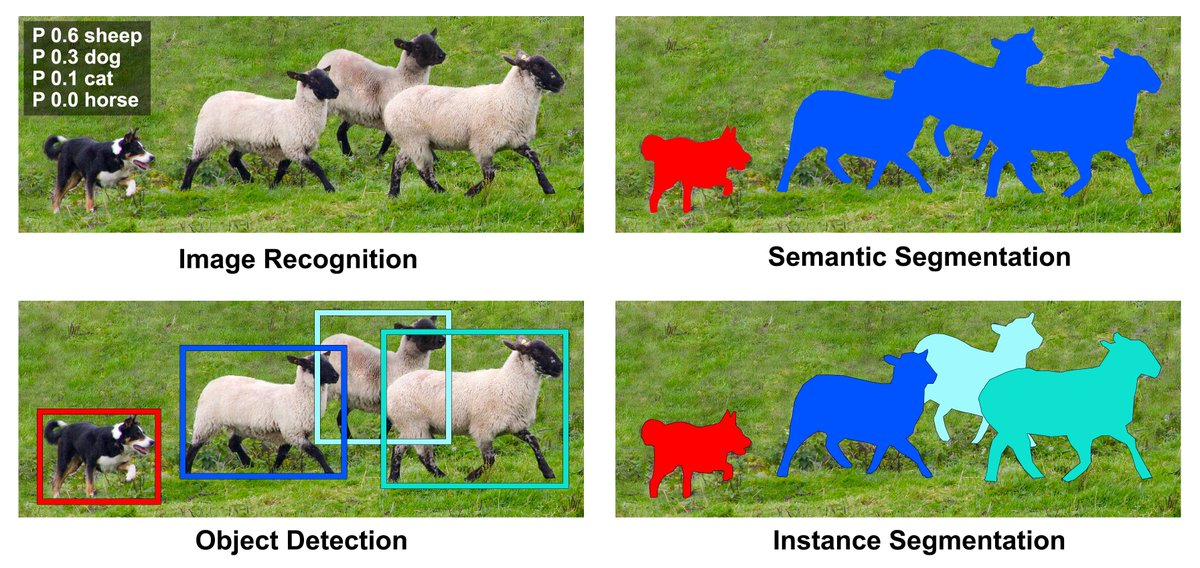
\includegraphics[width=10cm]{/home/thesis/images/Classification_vs_Segmentation.jpg}
    \caption{Illustration to compare different Machine vision tasks \cite{SemTorch76:online}. 
    Object detection means that the location of several objects is estimated by the model. This is indicated by the \textit{bounding boxes}.
    Segmentation of an image is classifying each pixel in the correct class or assigning it to the \textit{background} class.
    Semantic segmentation makes no difference between different instances of the same semantic class, instance segmentation does.
    \label{fig:machinevisiontasks}}
\end{SCfigure}

Other interesting applications of \gls{machinevision} include\footnote{This list is not exhaustive.}:
\begin{description}
    \item[Face recognition] is the identification of human faces. 
    \item[Image reconstruction] or \textit{inpainting} consists of recreating parts of a damaged image.
    \item[Image captioning] consists of the creation of full sentences describing the content of an image.    
\end{description}

\subsection{The convolution layer}

The building block of every modern machine vision network, including the ones in my thesis, is the convolution layer.

\todo[inline]{weight sharing, feature extraction}

\subsection{Data for training a machine vision model}

To perform the tasks discussed in chapter \ref{sec:machinevisiontasks}, one needs to build a suitable model.
For \Gls{machinevision} tasks\footnote{and many other tasks.}, the current standard approach is \Gls{deepl}.


The cost to generate, store and communicate images and computation power has dropped in the past decades.
This evolution allows to train a model  on previously unimaginable quantities of data\footnote{The \textit{ImageNet} database (\url{http://image-net.org/challenges/LSVRC/index}) consists of more than $14.10^6$ images.}.
This technique allows a model with a high number of degrees of freedom to be trainded\footnote{learn by example, so you will} without the need for expert-crafted features. 


Collection of this dataset - most importantly, the labels - proves to be a challenge. 
This chapter tries to explain what \textit{weak labels} and \textit{strong labels} are and what the difference is between both.

\subsubsection{Training a model}

To build a model to perform the tasks discussed in \ref{sec:machinevisiontasks}, this model needs to be trained.
This requires a set of \textit{labelled} images. 

In the classic approach, the supervision type closely resembles the intended model output.
To train a model that can classify an image\footnote{Given an image, the model outputs if this picture is a representation of class \textit{cat}, \textit{dog} or another animal or object. }, 
one has to \textit{train} the model on a set of labelled images where a human indicated the class.
To train a model to perform image segmentation\footnote{segmentation means that the model classifies each pixel.}, an expert needs to provide a set of images in which
each picture, the objects are delineated, indicating their class.  



\subsubsection{Weak supervision types}


To build a machine vision model, a collection of images is needed where an expert in the intended task has provided correct information from which the model can \textit{learn}.
Depending on the model objective, other types of labelling are required.


Figure \ref{fig:ImageLabelTypes} illustrates several types of image supervision : 
Point supervision, squiggle, bounding box and full mask.
The generation of these labels is costly and time-consuming.
Especially \gls{deepl} models are known to be very data-hungry. 

\begin{SCfigure}[][htb]
    \centering
    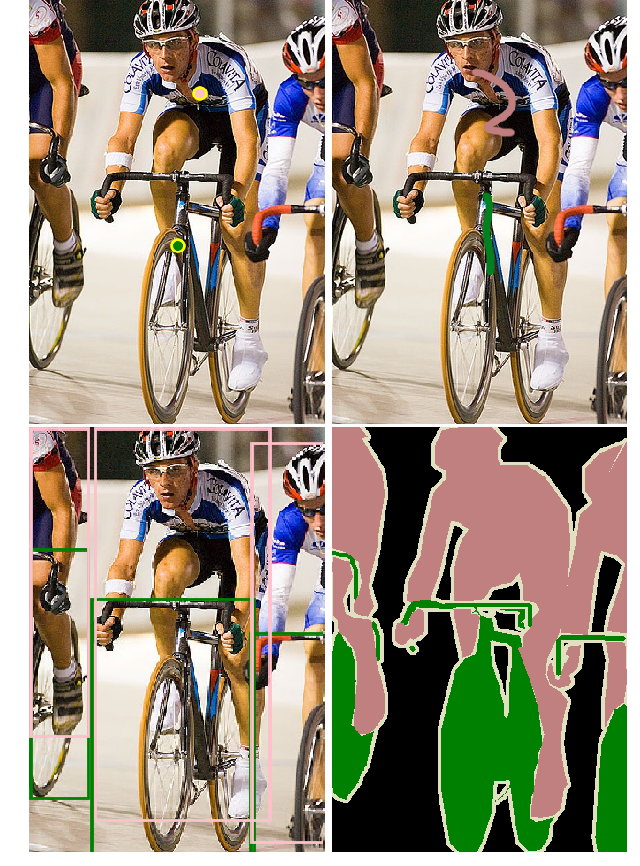
\includegraphics[width=10cm]{/home/thesis/images/McEver.png}
    \caption{Four different annotation types \cite{McEver2020}: 
    On the top left the picture is point level annotated. The points are inflated for visibility.
    On the top right, squiggle annotation is used.
    The bottom left shows bounding box supervion.
    While the bottom right image is fully annotated.
    An image level label would indicate that there are multiple instances of \textit{person} and \textit{bike} in the image.
    \label{fig:ImageLabelTypes}}
\end{SCfigure}

Given the high labelling cost, several researchers have investigated ways to train computer vision models with cheaper labels.
This branch of research is known as \Gls{weaklysupervisedl}.
The objective is to construct a robust model based on \textit{cheap} (incomplete, noisy or imprecise) labels. 
This is sometimes described as \textit{indirect supervision}.
Numerous creative approaches have been conceived. 
It is impossible to give an exhaustive list of approaches. 
In what follows, I will mainly focus on the approaches I chose to investigate myself, but I will also try to give some hints of the remarkable creativity found in the field.
Since the provided annotations in \Gls{weaklysupervisedl} are not full labels, these are sometimes described as \textit{hints} instead\footnote{
    This is based on the insightfull talk at \url{ 
        https://youtu.be/4EjYxVVCAaE
    }. For example, the destinction between labels and hints.
}.
The basic concept of \Gls{weaklysupervisedl} is that there are two sources of information to draw from: The hints and the prior knowledge about the problem (Priors).
These \textit{Priors} can be any form of prior knowledge about the object to be segmented\footnote{or any other machine vision task.}.
Priors can be the object size, shape or location, the number of instances, the similarity across images or the similarity with external images.

Whether an annotation is considered a \textit{weak label} or a \textit{strong label} depends more on the modellers intention than on the annotation itself. 
When one aims to construct a model to infer output labels with a higher informative value than the original annotations, these \textit{labels} become \textit{hints}.
Making a model predict bounding boxes from a dataset annotated with bounding boxes means considering these as \textit{strong labels}. 
If one uses the same dataset to construct a model that predicts pixel-wise masks, you use the labels as \textit{weak labels} or \textit{hints}.

For a segmentation task, weak labels can be:
\begin{description}
    \item[Image level labels]: When only  
\end{description}

\todo[inline]{Motivation of weakly supervised learning --> Difference in annotation time and cost from Bearman and Laradji Covid}